%#########################1########################

 \cajita{%
Hogares formales }%
{%
 }%
{%
 Hogares con viviendas formales según tipo de pobreza} %
{%
 República de Guatemala, 2014, en porcentaje} %
{%
 \begin{tikzpicture}[x=1pt,y=1pt]  % Created by tikzDevice version 0.9 on 2016-03-03 05:25:42
% !TEX encoding = UTF-8 Unicode
\definecolor{fillColor}{RGB}{255,255,255}
\path[use as bounding box,fill=fillColor,fill opacity=0.00] (0,0) rectangle (289.08,198.74);
\begin{scope}
\path[clip] (  0.00,  0.00) rectangle (289.08,198.74);

\path[] (  0.00,  0.00) rectangle (289.08,198.74);
\end{scope}
\begin{scope}
\path[clip] (  0.00,  0.00) rectangle (289.08,198.74);

\path[] ( -0.52, 15.61) rectangle (280.54,191.48);

\path[] (  0.00, 23.49) --
	(280.54, 23.49);

\path[] (  0.00, 71.25) --
	(280.54, 71.25);

\path[] (  0.00,119.01) --
	(280.54,119.01);

\path[] (  0.00,166.77) --
	(280.54,166.77);

\path[] (  0.00, 47.37) --
	(280.54, 47.37);

\path[] (  0.00, 95.13) --
	(280.54, 95.13);

\path[] (  0.00,142.89) --
	(280.54,142.89);

\path[] (  0.00,190.65) --
	(280.54,190.65);

\path[] ( 52.18, 15.61) --
	( 52.18,191.48);

\path[] (140.01, 15.61) --
	(140.01,191.48);

\path[] (227.84, 15.61) --
	(227.84,191.48);
\definecolor{drawColor}{RGB}{0,0,255}

\path[draw=drawColor,line width= 1.7pt,line join=round] ( 52.18, 60.50) --
	(140.01,141.70) --
	(227.84,183.49);
\definecolor{drawColor}{RGB}{0,0,0}

\node[text=drawColor,anchor=base,inner sep=0pt, outer sep=0pt, scale=  1.02] at ( 52.18, 48.59) {81.1};

\node[text=drawColor,anchor=base east,inner sep=0pt, outer sep=0pt, scale=  1.02] at (136.88,141.70) {87.9};

\node[text=drawColor,anchor=base,inner sep=0pt, outer sep=0pt, scale=  1.02] at (227.84,187.46) {91.4};

\path[draw=drawColor,line width= 0.1pt,line join=round] (  0.00, 23.61) -- (280.54, 23.61);

\path[] ( -0.52, 15.61) rectangle (280.54,191.48);
\end{scope}
\begin{scope}
\path[clip] (  0.00,  0.00) rectangle (289.08,198.74);

\path[] (  0.00, 15.61) --
	(280.54, 15.61);
\end{scope}
\begin{scope}
\path[clip] (  0.00,  0.00) rectangle (289.08,198.74);

\path[] ( 52.18, 12.86) --
	( 52.18, 15.61);

\path[] (140.01, 12.86) --
	(140.01, 15.61);

\path[] (227.84, 12.86) --
	(227.84, 15.61);
\end{scope}
\begin{scope}
\path[clip] (  0.00,  0.00) rectangle (289.08,198.74);
\definecolor{drawColor}{RGB}{0,0,0}

\node[text=drawColor,anchor=base,inner sep=0pt, outer sep=0pt, scale=  1.00] at ( 52.18,  2.85) {Pobreza Extrema};

\node[text=drawColor,anchor=base,inner sep=0pt, outer sep=0pt, scale=  1.00] at (140.01,  2.85) {Pobreza no extrema};

\node[text=drawColor,anchor=base,inner sep=0pt, outer sep=0pt, scale=  1.00] at (227.84,  2.85) {No pobreza};
\end{scope}
  \end{tikzpicture}}%
{%
 ENCOVI 2014} %

%#########################2########################

\cajita{%
	Viviendas con pared de block }%
{%
}%
{%
	Viviendas con pared de block según tipo de pobreza} %
{%
	República de Guatemala, 2014, en porcentaje} %
{%
	\begin{tikzpicture}[x=1pt,y=1pt]  % Created by tikzDevice version 0.9 on 2016-03-03 05:25:45
% !TEX encoding = UTF-8 Unicode
\definecolor{fillColor}{RGB}{255,255,255}
\path[use as bounding box,fill=fillColor,fill opacity=0.00] (0,0) rectangle (289.08,198.74);
\begin{scope}
\path[clip] (  0.00,  0.00) rectangle (289.08,198.74);

\path[] (  0.00,  0.00) rectangle (289.08,198.74);
\end{scope}
\begin{scope}
\path[clip] (  0.00,  0.00) rectangle (289.08,198.74);

\path[] ( -0.52, 15.61) rectangle (280.54,191.48);

\path[] (  0.00, 33.09) --
	(280.54, 33.09);

\path[] (  0.00, 78.90) --
	(280.54, 78.90);

\path[] (  0.00,124.70) --
	(280.54,124.70);

\path[] (  0.00,170.51) --
	(280.54,170.51);

\path[] (  0.00, 55.99) --
	(280.54, 55.99);

\path[] (  0.00,101.80) --
	(280.54,101.80);

\path[] (  0.00,147.61) --
	(280.54,147.61);

\path[] ( 52.18, 15.61) --
	( 52.18,191.48);

\path[] (140.01, 15.61) --
	(140.01,191.48);

\path[] (227.84, 15.61) --
	(227.84,191.48);
\definecolor{drawColor}{RGB}{0,0,255}

\path[draw=drawColor,line width= 1.7pt,line join=round] ( 52.18, 60.50) --
	(140.01,121.30) --
	(227.84,183.49);
\definecolor{drawColor}{RGB}{0,0,0}

\node[text=drawColor,anchor=base,inner sep=0pt, outer sep=0pt, scale=  1.02] at ( 52.18, 48.59) {22.0};

\node[text=drawColor,anchor=base east,inner sep=0pt, outer sep=0pt, scale=  1.02] at (136.88,121.30) {48.5};

\node[text=drawColor,anchor=base,inner sep=0pt, outer sep=0pt, scale=  1.02] at (227.84,187.46) {75.7};

\path[draw=drawColor,line width= 0.1pt,line join=round] (  0.00, 23.61) -- (280.54, 23.61);

\path[] ( -0.52, 15.61) rectangle (280.54,191.48);
\end{scope}
\begin{scope}
\path[clip] (  0.00,  0.00) rectangle (289.08,198.74);

\path[] (  0.00, 15.61) --
	(280.54, 15.61);
\end{scope}
\begin{scope}
\path[clip] (  0.00,  0.00) rectangle (289.08,198.74);

\path[] ( 52.18, 12.86) --
	( 52.18, 15.61);

\path[] (140.01, 12.86) --
	(140.01, 15.61);

\path[] (227.84, 12.86) --
	(227.84, 15.61);
\end{scope}
\begin{scope}
\path[clip] (  0.00,  0.00) rectangle (289.08,198.74);
\definecolor{drawColor}{RGB}{0,0,0}

\node[text=drawColor,anchor=base,inner sep=0pt, outer sep=0pt, scale=  1.00] at ( 52.18,  2.85) {Pobreza Extrema};

\node[text=drawColor,anchor=base,inner sep=0pt, outer sep=0pt, scale=  1.00] at (140.01,  2.85) {Pobreza no extrema};

\node[text=drawColor,anchor=base,inner sep=0pt, outer sep=0pt, scale=  1.00] at (227.84,  2.85) {No pobreza};
\end{scope}
  \end{tikzpicture}}%
{%
	ENCOVI 2014} %

%#########################3########################

\cajita{%
	Viviendas con techo de lámina }%
{%
}%
{%
	Viviendas con techo de lámina  según tipo de pobreza} %
{%
	República de Guatemala, 2014, en porcentaje} %
{%
	\begin{tikzpicture}[x=1pt,y=1pt]  % Created by tikzDevice version 0.9 on 2016-03-03 05:25:49
% !TEX encoding = UTF-8 Unicode
\definecolor{fillColor}{RGB}{255,255,255}
\path[use as bounding box,fill=fillColor,fill opacity=0.00] (0,0) rectangle (289.08,198.74);
\begin{scope}
\path[clip] (  0.00,  0.00) rectangle (289.08,198.74);

\path[] (  0.00,  0.00) rectangle (289.08,198.74);
\end{scope}
\begin{scope}
\path[clip] (  0.00,  0.00) rectangle (289.08,198.74);

\path[] ( -0.52, 15.61) rectangle (280.54,191.48);

\path[] (  0.00, 34.39) --
	(280.54, 34.39);

\path[] (  0.00, 62.22) --
	(280.54, 62.22);

\path[] (  0.00, 90.06) --
	(280.54, 90.06);

\path[] (  0.00,117.89) --
	(280.54,117.89);

\path[] (  0.00,145.72) --
	(280.54,145.72);

\path[] (  0.00,173.56) --
	(280.54,173.56);

\path[] (  0.00, 20.47) --
	(280.54, 20.47);

\path[] (  0.00, 48.31) --
	(280.54, 48.31);

\path[] (  0.00, 76.14) --
	(280.54, 76.14);

\path[] (  0.00,103.97) --
	(280.54,103.97);

\path[] (  0.00,131.81) --
	(280.54,131.81);

\path[] (  0.00,159.64) --
	(280.54,159.64);

\path[] (  0.00,187.47) --
	(280.54,187.47);

\path[] ( 52.18, 15.61) --
	( 52.18,191.48);

\path[] (140.01, 15.61) --
	(140.01,191.48);

\path[] (227.84, 15.61) --
	(227.84,191.48);
\definecolor{drawColor}{RGB}{0,0,255}

\path[draw=drawColor,line width= 1.7pt,line join=round] ( 52.18,183.49) --
	(140.01,172.52) --
	(227.84, 60.50);
\definecolor{drawColor}{RGB}{0,0,0}

\node[text=drawColor,anchor=base,inner sep=0pt, outer sep=0pt, scale=  1.02] at ( 52.18,187.46) {84.3};

\node[text=drawColor,anchor=base west,inner sep=0pt, outer sep=0pt, scale=  1.02] at (140.01,176.49) {82.3};

\node[text=drawColor,anchor=base,inner sep=0pt, outer sep=0pt, scale=  1.02] at (227.84, 48.59) {62.2};

\path[draw=drawColor,line width= 0.1pt,line join=round] (  0.00, 23.61) -- (280.54, 23.61);

\path[] ( -0.52, 15.61) rectangle (280.54,191.48);
\end{scope}
\begin{scope}
\path[clip] (  0.00,  0.00) rectangle (289.08,198.74);

\path[] (  0.00, 15.61) --
	(280.54, 15.61);
\end{scope}
\begin{scope}
\path[clip] (  0.00,  0.00) rectangle (289.08,198.74);

\path[] ( 52.18, 12.86) --
	( 52.18, 15.61);

\path[] (140.01, 12.86) --
	(140.01, 15.61);

\path[] (227.84, 12.86) --
	(227.84, 15.61);
\end{scope}
\begin{scope}
\path[clip] (  0.00,  0.00) rectangle (289.08,198.74);
\definecolor{drawColor}{RGB}{0,0,0}

\node[text=drawColor,anchor=base,inner sep=0pt, outer sep=0pt, scale=  1.00] at ( 52.18,  2.85) {Pobreza Extrema};

\node[text=drawColor,anchor=base,inner sep=0pt, outer sep=0pt, scale=  1.00] at (140.01,  2.85) {Pobreza no extrema};

\node[text=drawColor,anchor=base,inner sep=0pt, outer sep=0pt, scale=  1.00] at (227.84,  2.85) {No pobreza};
\end{scope}
  \end{tikzpicture}}%
{%
	ENCOVI 2014} %

%#########################4########################

\cajita{%
	Viviendas con material del piso}%
{%
}%
{%
	Viviendas según material del piso y tipo de pobreza} %
{%
	República de Guatemala, 2014, en porcentaje} %
{%
	\begin{tikzpicture}[x=1pt,y=1pt]  % Created by tikzDevice version 0.9 on 2016-03-03 05:25:52
% !TEX encoding = UTF-8 Unicode
\definecolor{fillColor}{RGB}{255,255,255}
\path[use as bounding box,fill=fillColor,fill opacity=0.00] (0,0) rectangle (289.08,198.74);
\begin{scope}
\path[clip] (  0.00,  0.00) rectangle (289.08,198.74);

\path[] (  0.00,  0.00) rectangle (289.08,198.74);
\end{scope}
\begin{scope}
\path[clip] (  0.00,  0.00) rectangle (289.08,198.74);

\path[] (  0.00, 18.46) rectangle (289.08,166.57);

\path[] ( 54.20, 18.46) --
	( 54.20,166.57);

\path[] (144.54, 18.46) --
	(144.54,166.57);

\path[] (234.88, 18.46) --
	(234.88,166.57);
\definecolor{drawColor}{RGB}{0,0,255}
\definecolor{fillColor}{RGB}{0,0,255}

\path[draw=drawColor,line width= 0.6pt,line join=round,fill=fillColor] ( 15.81, 18.46) rectangle ( 51.94, 74.33);
\definecolor{drawColor}{RGB}{157,187,255}
\definecolor{fillColor}{RGB}{157,187,255}

\path[draw=drawColor,line width= 0.6pt,line join=round,fill=fillColor] ( 56.46, 18.46) rectangle ( 92.60,166.57);
\definecolor{drawColor}{RGB}{0,0,255}
\definecolor{fillColor}{RGB}{0,0,255}

\path[draw=drawColor,line width= 0.6pt,line join=round,fill=fillColor] (106.15, 18.46) rectangle (142.28,120.72);
\definecolor{drawColor}{RGB}{157,187,255}
\definecolor{fillColor}{RGB}{157,187,255}

\path[draw=drawColor,line width= 0.6pt,line join=round,fill=fillColor] (146.80, 18.46) rectangle (182.93, 95.86);
\definecolor{drawColor}{RGB}{0,0,255}
\definecolor{fillColor}{RGB}{0,0,255}

\path[draw=drawColor,line width= 0.6pt,line join=round,fill=fillColor] (196.48, 18.46) rectangle (232.62,107.27);
\definecolor{drawColor}{RGB}{157,187,255}
\definecolor{fillColor}{RGB}{157,187,255}

\path[draw=drawColor,line width= 0.6pt,line join=round,fill=fillColor] (237.14, 18.46) rectangle (273.27, 41.36);
\definecolor{drawColor}{RGB}{0,0,0}

\path[draw=drawColor,line width= 0.6pt,line join=round] (  0.00, 18.46) -- (289.08, 18.46);

\node[text=drawColor,rotate= 90.00,anchor=base west,inner sep=0pt, outer sep=0pt, scale=  0.83] at ( 37.11, 76.88) {25.3};

\node[text=drawColor,rotate= 90.00,anchor=base west,inner sep=0pt, outer sep=0pt, scale=  0.83] at ( 77.76,169.12) {67.0};

\node[text=drawColor,rotate= 90.00,anchor=base west,inner sep=0pt, outer sep=0pt, scale=  0.83] at (127.45,123.26) {46.3};

\node[text=drawColor,rotate= 90.00,anchor=base west,inner sep=0pt, outer sep=0pt, scale=  0.83] at (168.10, 98.40) {35.0};

\node[text=drawColor,rotate= 90.00,anchor=base west,inner sep=0pt, outer sep=0pt, scale=  0.83] at (217.79,109.81) {40.2};

\node[text=drawColor,rotate= 90.00,anchor=base west,inner sep=0pt, outer sep=0pt, scale=  0.83] at (258.44, 43.91) {10.4};

\path[] (  0.00, 18.46) rectangle (289.08,166.57);
\end{scope}
\begin{scope}
\path[clip] (  0.00,  0.00) rectangle (289.08,198.74);

\path[] (  0.00, 18.46) --
	(289.08, 18.46);
\end{scope}
\begin{scope}
\path[clip] (  0.00,  0.00) rectangle (289.08,198.74);

\path[] ( 54.20, 15.71) --
	( 54.20, 18.46);

\path[] (144.54, 15.71) --
	(144.54, 18.46);

\path[] (234.88, 15.71) --
	(234.88, 18.46);
\end{scope}
\begin{scope}
\path[clip] (  0.00,  0.00) rectangle (289.08,198.74);
\definecolor{drawColor}{RGB}{0,0,0}

\node[text=drawColor,anchor=base,inner sep=0pt, outer sep=0pt, scale=  1.00] at ( 54.20,  5.69) {Pobreza Extrema};

\node[text=drawColor,anchor=base,inner sep=0pt, outer sep=0pt, scale=  1.00] at (144.54,  5.69) {Pobreza no extrema};

\node[text=drawColor,anchor=base,inner sep=0pt, outer sep=0pt, scale=  1.00] at (234.88,  5.69) {No pobreza};
\end{scope}
\begin{scope}
\path[clip] (  0.00,  0.00) rectangle (289.08,198.74);
\coordinate (apoyo) at (41.26,191.13);
\coordinate (longitudFicticia) at (7.11,7.61);
\coordinate (longitud) at (7.11,7.11);
\coordinate (desX) at (157.45,0);
\coordinate (desY) at (0,0.25);
\definecolor[named]{ct1}{HTML}{
0000FF
}
\definecolor[named]{ct2}{HTML}{
9DBBFF
}
\definecolor[named]{ctb1}{HTML}{
0000FF
}
\definecolor[named]{ctb2}{HTML}{
9DBBFF
}
\path [fill=none] (apoyo) rectangle ($(apoyo)+(longitudFicticia)$)
node [xshift=0.3cm,inner sep=0pt, outer sep=0pt,midway,right,scale = 0.9]{Torta de cemento};
\draw [color = ctb1,fill=ct1] ( $(apoyo)  + (desY) $) rectangle ($(apoyo)+ (desY) +(longitud)$);
\path [fill=none] ($(apoyo)+(desX)$) rectangle ($(apoyo)+(desX)+(longitudFicticia)$)
node [xshift=0.3cm,inner sep=0pt, outer sep=0pt,midway,right,scale = 0.9]{Tierra};
\draw [color = ctb2 ,fill=ct2] ( $(apoyo)  + (desY) + (desX) $) rectangle ($(apoyo)+ (desY)+ (desX) +(longitud)$);
\end{scope}
  \end{tikzpicture}}%
{%
	ENCOVI 2014} %

%#########################5########################

\cajita{%
	Viviendas y acceso al agua}%
{%
}%
{%
	Viviendas que tienen acceso a agua según area de residencia} %
{%
	República de Guatemala, 2014, en porcentaje} %
{%
	\begin{tikzpicture}[x=1pt,y=1pt]  \input{graficas/5_05.tex}  \end{tikzpicture}}%
{%
	ENCOVI 2014} %


%#########################6########################

\cajita{%
	Viviendas y acceso a drenajes}%
{%
}%
{%
	Viviendas que tienen acceso a drenajes según area de residencia} %
{%
	República de Guatemala, 2014, en porcentaje} %
{%
	\begin{tikzpicture}[x=1pt,y=1pt]  \input{graficas/5_06.tex}  \end{tikzpicture}}%
{%
	ENCOVI 2014} %

%#########################7########################

\cajita{%
	TGF}%
{%
}%
{%
	Evolución de la tasa global de fecundidad} %
{%
	República de Guatemala, serie histórica, niños por mujer} %
{%
	\begin{tikzpicture}[x=1pt,y=1pt]  % Created by tikzDevice version 0.9 on 2016-03-03 05:26:08
% !TEX encoding = UTF-8 Unicode
\definecolor{fillColor}{RGB}{255,255,255}
\path[use as bounding box,fill=fillColor,fill opacity=0.00] (0,0) rectangle (289.08,198.74);
\begin{scope}
\path[clip] (  0.00,  0.00) rectangle (289.08,198.74);

\path[] (  0.00,  0.00) rectangle (289.08,198.74);
\end{scope}
\begin{scope}
\path[clip] (  0.00,  0.00) rectangle (289.08,198.74);

\path[] (  1.74, 15.61) rectangle (280.54,191.48);

\path[] (  1.74, 38.98) --
	(280.54, 38.98);

\path[] (  1.74, 69.73) --
	(280.54, 69.73);

\path[] (  1.74,100.47) --
	(280.54,100.47);

\path[] (  1.74,131.22) --
	(280.54,131.22);

\path[] (  1.74,161.97) --
	(280.54,161.97);

\path[] (  1.74, 23.61) --
	(280.54, 23.61);

\path[] (  1.74, 54.35) --
	(280.54, 54.35);

\path[] (  1.74, 85.10) --
	(280.54, 85.10);

\path[] (  1.74,115.85) --
	(280.54,115.85);

\path[] (  1.74,146.59) --
	(280.54,146.59);

\path[] (  1.74,177.34) --
	(280.54,177.34);

\path[] ( 41.57, 15.61) --
	( 41.57,191.48);

\path[] (107.95, 15.61) --
	(107.95,191.48);

\path[] (174.33, 15.61) --
	(174.33,191.48);

\path[] (240.71, 15.61) --
	(240.71,191.48);
\definecolor{drawColor}{RGB}{0,0,255}

\path[draw=drawColor,line width= 1.7pt,line join=round] ( 41.57,183.49) --
	(107.95,140.44) --
	(174.33, 91.25) --
	(240.71, 60.50);
\definecolor{drawColor}{RGB}{0,0,0}

\node[text=drawColor,anchor=base,inner sep=0pt, outer sep=0pt, scale=  1.02] at ( 41.57,187.46) {5.1};

\node[text=drawColor,anchor=base west,inner sep=0pt, outer sep=0pt, scale=  1.02] at (107.95,144.41) {4.4};

\node[text=drawColor,anchor=base west,inner sep=0pt, outer sep=0pt, scale=  1.02] at (174.33, 95.22) {3.6};

\node[text=drawColor,anchor=base,inner sep=0pt, outer sep=0pt, scale=  1.02] at (240.71, 48.59) {3.1};

\path[draw=drawColor,line width= 0.1pt,line join=round] (  1.74, 23.61) -- (280.54, 23.61);

\path[] (  1.74, 15.61) rectangle (280.54,191.48);
\end{scope}
\begin{scope}
\path[clip] (  0.00,  0.00) rectangle (289.08,198.74);

\path[] (  1.74, 15.61) --
	(  1.74,191.48);
\end{scope}
\begin{scope}
\path[clip] (  0.00,  0.00) rectangle (289.08,198.74);

\path[] (  0.00, 23.61) --
	(  1.74, 23.61);

\path[] (  0.00, 54.35) --
	(  1.74, 54.35);

\path[] (  0.00, 85.10) --
	(  1.74, 85.10);

\path[] (  0.00,115.85) --
	(  1.74,115.85);

\path[] (  0.00,146.59) --
	(  1.74,146.59);

\path[] (  0.00,177.34) --
	(  1.74,177.34);
\end{scope}
\begin{scope}
\path[clip] (  0.00,  0.00) rectangle (289.08,198.74);

\path[] (  1.74, 15.61) --
	(280.54, 15.61);
\end{scope}
\begin{scope}
\path[clip] (  0.00,  0.00) rectangle (289.08,198.74);

\path[] ( 41.57, 12.86) --
	( 41.57, 15.61);

\path[] (107.95, 12.86) --
	(107.95, 15.61);

\path[] (174.33, 12.86) --
	(174.33, 15.61);

\path[] (240.71, 12.86) --
	(240.71, 15.61);
\end{scope}
\begin{scope}
\path[clip] (  0.00,  0.00) rectangle (289.08,198.74);
\definecolor{drawColor}{RGB}{0,0,0}

\node[text=drawColor,anchor=base,inner sep=0pt, outer sep=0pt, scale=  1.00] at ( 41.57,  2.85) {1995};

\node[text=drawColor,anchor=base,inner sep=0pt, outer sep=0pt, scale=  1.00] at (107.95,  2.85) {2002};

\node[text=drawColor,anchor=base,inner sep=0pt, outer sep=0pt, scale=  1.00] at (174.33,  2.85) {2008-2009};

\node[text=drawColor,anchor=base,inner sep=0pt, outer sep=0pt, scale=  1.00] at (240.71,  2.85) {2014-2015};
\end{scope}
  \end{tikzpicture}}%
{%
	ENSMI 2014, 2008, 2002 y 1995} %

%#########################8########################

\cajita{%
	TGF por área de residencia}%
{%
}%
{%
	Tasa global de fecundidad por área de residencia} %
{%
	República de Guatemala, 2014, niños por mujer} %
{%
	\begin{tikzpicture}[x=1pt,y=1pt]  \input{graficas/5_08.tex}  \end{tikzpicture}}%
{%
	ENSMI 2014, 2008, 2002 y 1995} %



%#########################9########################

\cajita{%
	Asistencia prenatal}%
{%
}%
{%
	Mujeres que recibieron atención prenatal de un proveedor calificado} %
{%
	República de Guatemala, 2014, en porcentaje} %
{%
	\begin{tikzpicture}[x=1pt,y=1pt]  \input{graficas/5_09.tex}  \end{tikzpicture}}%
{%
	ENSMI 2014} %

%#########################10########################

\cajita{%
	Asistencia en el parto}%
{%
}%
{%
	Mujeres que recibieron atención a la hora del parto  de un proveedor calificado} %
{%
	República de Guatemala, 2014, en porcentaje} %
{%
	\begin{tikzpicture}[x=1pt,y=1pt]  \input{graficas/5_10.tex}  \end{tikzpicture}}%
{%
	ENSMI 2014} %

%#########################11########################

\cajita{%
	Niños que reciben alguna vacuna o desparasitante}%
{%
}%
{%
	Niños que reciben vacunas o desparasitante} %
{%
	República de Guatemala, serie histórica, número de niños} %
{%
	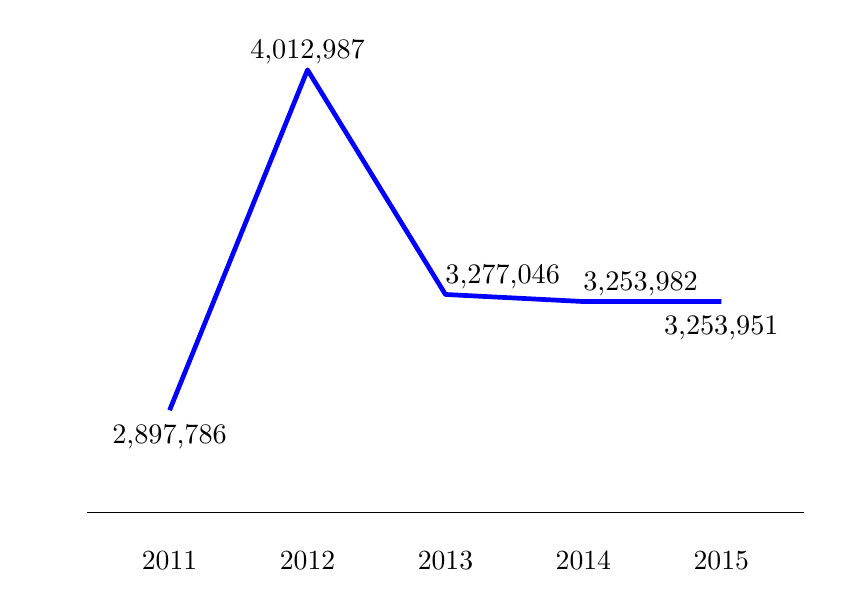
\begin{tikzpicture}[x=1pt,y=1pt]  % Created by tikzDevice version 0.9 on 2016-03-03 05:26:22
% !TEX encoding = UTF-8 Unicode
\definecolor{fillColor}{RGB}{255,255,255}
\path[use as bounding box,fill=fillColor,fill opacity=0.00] (0,0) rectangle (289.08,198.74);
\begin{scope}
\path[clip] (  0.00,  0.00) rectangle (289.08,198.74);

\path[] (  0.00,  0.00) rectangle (289.08,198.74);
\end{scope}
\begin{scope}
\path[clip] (  0.00,  0.00) rectangle (289.08,198.74);

\path[] ( 21.38, 15.61) rectangle (280.54,191.48);

\path[] ( 21.38, 44.20) --
	(280.54, 44.20);

\path[] ( 21.38, 99.35) --
	(280.54, 99.35);

\path[] ( 21.38,154.49) --
	(280.54,154.49);

\path[] ( 21.38, 16.63) --
	(280.54, 16.63);

\path[] ( 21.38, 71.77) --
	(280.54, 71.77);

\path[] ( 21.38,126.92) --
	(280.54,126.92);

\path[] ( 21.38,182.06) --
	(280.54,182.06);

\path[] ( 51.28, 15.61) --
	( 51.28,191.48);

\path[] (101.12, 15.61) --
	(101.12,191.48);

\path[] (150.96, 15.61) --
	(150.96,191.48);

\path[] (200.80, 15.61) --
	(200.80,191.48);

\path[] (250.64, 15.61) --
	(250.64,191.48);
\definecolor{drawColor}{RGB}{0,0,255}

\path[draw=drawColor,line width= 1.7pt,line join=round] ( 51.28, 60.50) --
	(101.12,183.49) --
	(150.96,102.33) --
	(200.80, 99.78) --
	(250.64, 99.78);
\definecolor{drawColor}{RGB}{0,0,0}

\node[text=drawColor,anchor=base,inner sep=0pt, outer sep=0pt, scale=  1.02] at ( 51.28, 48.59) {2,897,786};

\node[text=drawColor,anchor=base,inner sep=0pt, outer sep=0pt, scale=  1.02] at (101.12,187.46) {4,012,987};

\node[text=drawColor,anchor=base west,inner sep=0pt, outer sep=0pt, scale=  1.02] at (150.96,106.30) {3,277,046};

\node[text=drawColor,anchor=base west,inner sep=0pt, outer sep=0pt, scale=  1.02] at (200.80,103.76) {3,253,982};

\node[text=drawColor,anchor=base,inner sep=0pt, outer sep=0pt, scale=  1.02] at (250.64, 87.87) {3,253,951};

\path[draw=drawColor,line width= 0.1pt,line join=round] ( 21.38, 23.61) -- (280.54, 23.61);

\path[] ( 21.38, 15.61) rectangle (280.54,191.48);
\end{scope}
\begin{scope}
\path[clip] (  0.00,  0.00) rectangle (289.08,198.74);

\path[] ( 21.38, 15.61) --
	( 21.38,191.48);
\end{scope}
\begin{scope}
\path[clip] (  0.00,  0.00) rectangle (289.08,198.74);
\definecolor{drawColor}{RGB}{255,255,255}

\node[text=drawColor,text opacity=0.00,anchor=base east,inner sep=0pt, outer sep=0pt, scale=  1.00] at ( 16.43, 12.73) {2500000};

\node[text=drawColor,text opacity=0.00,anchor=base east,inner sep=0pt, outer sep=0pt, scale=  1.00] at ( 16.43, 67.87) {3000000};

\node[text=drawColor,text opacity=0.00,anchor=base east,inner sep=0pt, outer sep=0pt, scale=  1.00] at ( 16.43,123.01) {3500000};

\node[text=drawColor,text opacity=0.00,anchor=base east,inner sep=0pt, outer sep=0pt, scale=  1.00] at ( 16.43,178.15) {4000000};
\end{scope}
\begin{scope}
\path[clip] (  0.00,  0.00) rectangle (289.08,198.74);

\path[] ( 18.63, 16.63) --
	( 21.38, 16.63);

\path[] ( 18.63, 71.77) --
	( 21.38, 71.77);

\path[] ( 18.63,126.92) --
	( 21.38,126.92);

\path[] ( 18.63,182.06) --
	( 21.38,182.06);
\end{scope}
\begin{scope}
\path[clip] (  0.00,  0.00) rectangle (289.08,198.74);

\path[] ( 21.38, 15.61) --
	(280.54, 15.61);
\end{scope}
\begin{scope}
\path[clip] (  0.00,  0.00) rectangle (289.08,198.74);

\path[] ( 51.28, 12.86) --
	( 51.28, 15.61);

\path[] (101.12, 12.86) --
	(101.12, 15.61);

\path[] (150.96, 12.86) --
	(150.96, 15.61);

\path[] (200.80, 12.86) --
	(200.80, 15.61);

\path[] (250.64, 12.86) --
	(250.64, 15.61);
\end{scope}
\begin{scope}
\path[clip] (  0.00,  0.00) rectangle (289.08,198.74);
\definecolor{drawColor}{RGB}{0,0,0}

\node[text=drawColor,anchor=base,inner sep=0pt, outer sep=0pt, scale=  1.00] at ( 51.28,  2.85) {2011};

\node[text=drawColor,anchor=base,inner sep=0pt, outer sep=0pt, scale=  1.00] at (101.12,  2.85) {2012};

\node[text=drawColor,anchor=base,inner sep=0pt, outer sep=0pt, scale=  1.00] at (150.96,  2.85) {2013};

\node[text=drawColor,anchor=base,inner sep=0pt, outer sep=0pt, scale=  1.00] at (200.80,  2.85) {2014};

\node[text=drawColor,anchor=base,inner sep=0pt, outer sep=0pt, scale=  1.00] at (250.64,  2.85) {2015};
\end{scope}
  \end{tikzpicture}}%
{%
	SIGSA} %

%#########################12########################

\cajita{%
	Diarrea}%
{%
}%
{%
	Niños menores de cinco años que recibieron atención médica por diarrea} %
{%
	República de Guatemala, serie histórica, número de niños} %
{%
	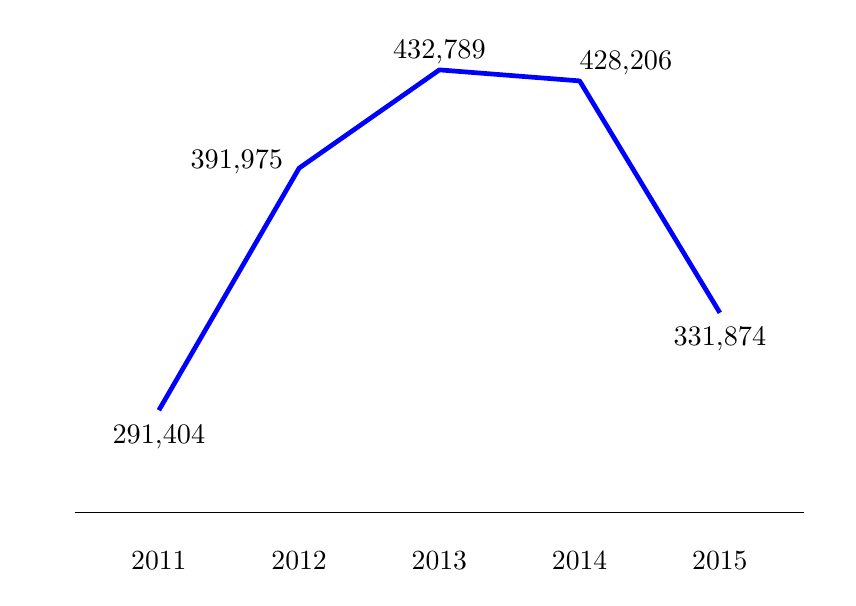
\begin{tikzpicture}[x=1pt,y=1pt]  % Created by tikzDevice version 0.9 on 2016-03-03 05:26:29
% !TEX encoding = UTF-8 Unicode
\definecolor{fillColor}{RGB}{255,255,255}
\path[use as bounding box,fill=fillColor,fill opacity=0.00] (0,0) rectangle (289.08,198.74);
\begin{scope}
\path[clip] (  0.00,  0.00) rectangle (289.08,198.74);

\path[] (  0.00,  0.00) rectangle (289.08,198.74);
\end{scope}
\begin{scope}
\path[clip] (  0.00,  0.00) rectangle (289.08,198.74);

\path[] ( 17.00, 15.61) rectangle (280.54,191.48);

\path[] ( 17.00, 46.23) --
	(280.54, 46.23);

\path[] ( 17.00, 89.73) --
	(280.54, 89.73);

\path[] ( 17.00,133.22) --
	(280.54,133.22);

\path[] ( 17.00,176.71) --
	(280.54,176.71);

\path[] ( 17.00, 24.49) --
	(280.54, 24.49);

\path[] ( 17.00, 67.98) --
	(280.54, 67.98);

\path[] ( 17.00,111.47) --
	(280.54,111.47);

\path[] ( 17.00,154.97) --
	(280.54,154.97);

\path[] ( 47.41, 15.61) --
	( 47.41,191.48);

\path[] ( 98.09, 15.61) --
	( 98.09,191.48);

\path[] (148.77, 15.61) --
	(148.77,191.48);

\path[] (199.45, 15.61) --
	(199.45,191.48);

\path[] (250.13, 15.61) --
	(250.13,191.48);
\definecolor{drawColor}{RGB}{0,0,255}

\path[draw=drawColor,line width= 1.7pt,line join=round] ( 47.41, 60.50) --
	( 98.09,147.99) --
	(148.77,183.49) --
	(199.45,179.50) --
	(250.13, 95.71);
\definecolor{drawColor}{RGB}{0,0,0}

\node[text=drawColor,anchor=base,inner sep=0pt, outer sep=0pt, scale=  1.02] at ( 47.41, 48.59) {291,404};

\node[text=drawColor,anchor=base east,inner sep=0pt, outer sep=0pt, scale=  1.02] at ( 92.29,147.99) {391,975};

\node[text=drawColor,anchor=base,inner sep=0pt, outer sep=0pt, scale=  1.02] at (148.77,187.46) {432,789};

\node[text=drawColor,anchor=base west,inner sep=0pt, outer sep=0pt, scale=  1.02] at (199.45,183.47) {428,206};

\node[text=drawColor,anchor=base,inner sep=0pt, outer sep=0pt, scale=  1.02] at (250.13, 83.79) {331,874};

\path[draw=drawColor,line width= 0.1pt,line join=round] ( 17.00, 23.61) -- (280.54, 23.61);

\path[] ( 17.00, 15.61) rectangle (280.54,191.48);
\end{scope}
\begin{scope}
\path[clip] (  0.00,  0.00) rectangle (289.08,198.74);

\path[] ( 17.00, 15.61) --
	( 17.00,191.48);
\end{scope}
\begin{scope}
\path[clip] (  0.00,  0.00) rectangle (289.08,198.74);
\definecolor{drawColor}{RGB}{255,255,255}

\node[text=drawColor,text opacity=0.00,anchor=base east,inner sep=0pt, outer sep=0pt, scale=  1.00] at ( 12.05, 20.58) {250000};

\node[text=drawColor,text opacity=0.00,anchor=base east,inner sep=0pt, outer sep=0pt, scale=  1.00] at ( 12.05, 64.07) {300000};

\node[text=drawColor,text opacity=0.00,anchor=base east,inner sep=0pt, outer sep=0pt, scale=  1.00] at ( 12.05,107.56) {350000};

\node[text=drawColor,text opacity=0.00,anchor=base east,inner sep=0pt, outer sep=0pt, scale=  1.00] at ( 12.05,151.06) {400000};
\end{scope}
\begin{scope}
\path[clip] (  0.00,  0.00) rectangle (289.08,198.74);

\path[] ( 14.25, 24.49) --
	( 17.00, 24.49);

\path[] ( 14.25, 67.98) --
	( 17.00, 67.98);

\path[] ( 14.25,111.47) --
	( 17.00,111.47);

\path[] ( 14.25,154.97) --
	( 17.00,154.97);
\end{scope}
\begin{scope}
\path[clip] (  0.00,  0.00) rectangle (289.08,198.74);

\path[] ( 17.00, 15.61) --
	(280.54, 15.61);
\end{scope}
\begin{scope}
\path[clip] (  0.00,  0.00) rectangle (289.08,198.74);

\path[] ( 47.41, 12.86) --
	( 47.41, 15.61);

\path[] ( 98.09, 12.86) --
	( 98.09, 15.61);

\path[] (148.77, 12.86) --
	(148.77, 15.61);

\path[] (199.45, 12.86) --
	(199.45, 15.61);

\path[] (250.13, 12.86) --
	(250.13, 15.61);
\end{scope}
\begin{scope}
\path[clip] (  0.00,  0.00) rectangle (289.08,198.74);
\definecolor{drawColor}{RGB}{0,0,0}

\node[text=drawColor,anchor=base,inner sep=0pt, outer sep=0pt, scale=  1.00] at ( 47.41,  2.85) {2011};

\node[text=drawColor,anchor=base,inner sep=0pt, outer sep=0pt, scale=  1.00] at ( 98.09,  2.85) {2012};

\node[text=drawColor,anchor=base,inner sep=0pt, outer sep=0pt, scale=  1.00] at (148.77,  2.85) {2013};

\node[text=drawColor,anchor=base,inner sep=0pt, outer sep=0pt, scale=  1.00] at (199.45,  2.85) {2014};

\node[text=drawColor,anchor=base,inner sep=0pt, outer sep=0pt, scale=  1.00] at (250.13,  2.85) {2015};
\end{scope}
  \end{tikzpicture}}%
{%
	SIGSA} %

%#########################13########################

\cajita{%
	Diarrea según sexo}%
{%
}%
{%
	Niños menores de cinco años que recibieron atención médica por diarrea según sexo} %
{%
	República de Guatemala, 2015, número de niños} %
{%
	\begin{tikzpicture}[x=1pt,y=1pt]  \input{graficas/5_13.tex}  \end{tikzpicture}}%
{%
	SIGSA} %

%#########################14########################

\cajota{%
 Casos de diarrea por departamento}%
{%
}%
{%
	Niños menores de cinco años que recibieron atención médica por diarrea por departamento} %
{%
	República de Guatemala, departamental, número de niños} %
{%
	\includegraphics[width=52\cuadri]{graficas/5_14.pdf}}%
{%
	SIGSA} %

%#########################15########################

\cajita{%
	Infecciones respiratorias agudas}%
{%
}%
{%
	Niños menores de cinco años que recibieron atención médica por infecciones respiratorias agudas} %
{%
	República de Guatemala, serie histórica, número de niños} %
{%
	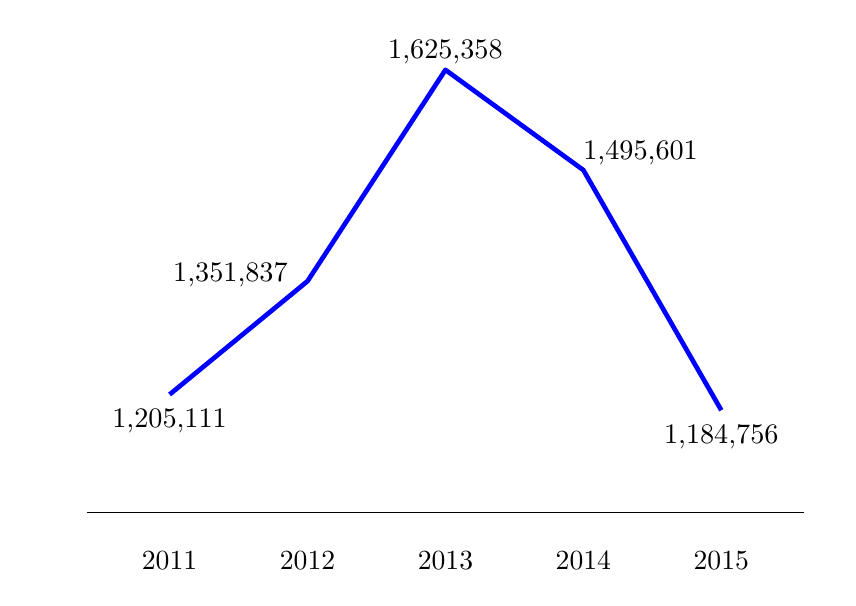
\begin{tikzpicture}[x=1pt,y=1pt]  % Created by tikzDevice version 0.9 on 2016-03-03 05:26:40
% !TEX encoding = UTF-8 Unicode
\definecolor{fillColor}{RGB}{255,255,255}
\path[use as bounding box,fill=fillColor,fill opacity=0.00] (0,0) rectangle (289.08,198.74);
\begin{scope}
\path[clip] (  0.00,  0.00) rectangle (289.08,198.74);

\path[] (  0.00,  0.00) rectangle (289.08,198.74);
\end{scope}
\begin{scope}
\path[clip] (  0.00,  0.00) rectangle (289.08,198.74);

\path[] ( 21.38, 15.61) rectangle (280.54,191.48);

\path[] ( 21.38, 36.84) --
	(280.54, 36.84);

\path[] ( 21.38, 92.67) --
	(280.54, 92.67);

\path[] ( 21.38,148.50) --
	(280.54,148.50);

\path[] ( 21.38, 64.76) --
	(280.54, 64.76);

\path[] ( 21.38,120.58) --
	(280.54,120.58);

\path[] ( 21.38,176.41) --
	(280.54,176.41);

\path[] ( 51.28, 15.61) --
	( 51.28,191.48);

\path[] (101.12, 15.61) --
	(101.12,191.48);

\path[] (150.96, 15.61) --
	(150.96,191.48);

\path[] (200.80, 15.61) --
	(200.80,191.48);

\path[] (250.64, 15.61) --
	(250.64,191.48);
\definecolor{drawColor}{RGB}{0,0,255}

\path[draw=drawColor,line width= 1.7pt,line join=round] ( 51.28, 66.18) --
	(101.12,107.14) --
	(150.96,183.49) --
	(200.80,147.27) --
	(250.64, 60.50);
\definecolor{drawColor}{RGB}{0,0,0}

\node[text=drawColor,anchor=base,inner sep=0pt, outer sep=0pt, scale=  1.02] at ( 51.28, 54.27) {1,205,111};

\node[text=drawColor,anchor=base east,inner sep=0pt, outer sep=0pt, scale=  1.02] at ( 93.97,107.14) {1,351,837};

\node[text=drawColor,anchor=base,inner sep=0pt, outer sep=0pt, scale=  1.02] at (150.96,187.46) {1,625,358};

\node[text=drawColor,anchor=base west,inner sep=0pt, outer sep=0pt, scale=  1.02] at (200.80,151.24) {1,495,601};

\node[text=drawColor,anchor=base,inner sep=0pt, outer sep=0pt, scale=  1.02] at (250.64, 48.59) {1,184,756};

\path[draw=drawColor,line width= 0.1pt,line join=round] ( 21.38, 23.61) -- (280.54, 23.61);

\path[] ( 21.38, 15.61) rectangle (280.54,191.48);
\end{scope}
\begin{scope}
\path[clip] (  0.00,  0.00) rectangle (289.08,198.74);

\path[] ( 21.38, 15.61) --
	( 21.38,191.48);
\end{scope}
\begin{scope}
\path[clip] (  0.00,  0.00) rectangle (289.08,198.74);
\definecolor{drawColor}{RGB}{255,255,255}

\node[text=drawColor,text opacity=0.00,anchor=base east,inner sep=0pt, outer sep=0pt, scale=  1.00] at ( 16.43, 60.85) {1200000};

\node[text=drawColor,text opacity=0.00,anchor=base east,inner sep=0pt, outer sep=0pt, scale=  1.00] at ( 16.43,116.68) {1400000};

\node[text=drawColor,text opacity=0.00,anchor=base east,inner sep=0pt, outer sep=0pt, scale=  1.00] at ( 16.43,172.50) {1600000};
\end{scope}
\begin{scope}
\path[clip] (  0.00,  0.00) rectangle (289.08,198.74);

\path[] ( 18.63, 64.76) --
	( 21.38, 64.76);

\path[] ( 18.63,120.58) --
	( 21.38,120.58);

\path[] ( 18.63,176.41) --
	( 21.38,176.41);
\end{scope}
\begin{scope}
\path[clip] (  0.00,  0.00) rectangle (289.08,198.74);

\path[] ( 21.38, 15.61) --
	(280.54, 15.61);
\end{scope}
\begin{scope}
\path[clip] (  0.00,  0.00) rectangle (289.08,198.74);

\path[] ( 51.28, 12.86) --
	( 51.28, 15.61);

\path[] (101.12, 12.86) --
	(101.12, 15.61);

\path[] (150.96, 12.86) --
	(150.96, 15.61);

\path[] (200.80, 12.86) --
	(200.80, 15.61);

\path[] (250.64, 12.86) --
	(250.64, 15.61);
\end{scope}
\begin{scope}
\path[clip] (  0.00,  0.00) rectangle (289.08,198.74);
\definecolor{drawColor}{RGB}{0,0,0}

\node[text=drawColor,anchor=base,inner sep=0pt, outer sep=0pt, scale=  1.00] at ( 51.28,  2.85) {2011};

\node[text=drawColor,anchor=base,inner sep=0pt, outer sep=0pt, scale=  1.00] at (101.12,  2.85) {2012};

\node[text=drawColor,anchor=base,inner sep=0pt, outer sep=0pt, scale=  1.00] at (150.96,  2.85) {2013};

\node[text=drawColor,anchor=base,inner sep=0pt, outer sep=0pt, scale=  1.00] at (200.80,  2.85) {2014};

\node[text=drawColor,anchor=base,inner sep=0pt, outer sep=0pt, scale=  1.00] at (250.64,  2.85) {2015};
\end{scope}
  \end{tikzpicture}}%
{%
	SIGSA} %

%#########################16########################

\cajita{%
	Infecciones respiratorias agudas según sexo}%
{%
}%
{%
	Niños menores de cinco años que recibieron atención médica por infecciones respiratorias agudas según sexo} %
{%
	República de Guatemala, 2015, número de niños} %
{%
	\begin{tikzpicture}[x=1pt,y=1pt]  \input{graficas/5_16.tex}  \end{tikzpicture}}%
{%
	SIGSA} %

%#########################17########################

\cajota{%
	Casos de IRA por departamento}%
{%
}%
{%
	Niños menores de cinco años que recibieron atención médica por infecciones respiratorias agudas por departamento} %
{%
	República de Guatemala, departamental, número de niños} %
{%
	\includegraphics[width=52\cuadri]{graficas/5_17.pdf}}%
{%
	SIGSA} %
